We developed ORES in the context of Wikipedia, which generally sees itself as an egalitarian, decentralized, and radically transparent community.  With ORES, we sought to maintain these values in our system design and model building strategies.  The flow of data --- from random samples through model training, evaluation, and application --- is open for review, critique, and iteration.  We have also developed novel strategies for opening ORES models up to evaluation, experimentation, and play based on user requests.  In this section, we describe some of the key, novel innovations that have made ORES fit Wikipedian concerns and be flexible to re-appropriation.  Section~\ref{sec:appendix} also contains information about ORES' detailed prediction output, how users and tools can adjust their use to model fitness, and how the whole model development workflow is made inspectable and replicable.

\subsection{Collaboratively labeled data}
There are two primary strategies for gathering labeled data for ORES' models: found traces and manual labels.

\leadin{Found traces} For many models, the MediaWiki platform records a rich set of digital traces that can be assumed to reflect a useful human judgement for modeling.  For example, in Wikipedia, it is very common that damaging edits will eventually be reverted\footnote{In Wikipedian parlance, a ``revert'' is a direct undoing of an edit, bringing the article to the exact same state it was in before.} and that good edits will not be reverted.  Thus the revert action (and remaining traces) can be used as an endogenous label in training.  We have developed a re-usable script\footnote{see \emph{autolabel} in \url{https://github.com/wiki-ai/editquality}} that when given a sample of edits, will label the edits as ``reverted\_for\_damage'' or not based on a set of constraints: the edit was reverted within 48 hours, the reverting editor was not the original editor, and the edit was not later restored by someone other than the original editor.

However, this ``reverted\_for\_damage'' label is problematic in that many edits are reverted not because they are damaging, but instead because they are tied up in an editorial dispute.  Operationalizing quality by exclusively measuring what persists in Wikipedia reinforces Wikipedia's well-known systemic biases, which is a similar problem in using found crime data in predictive policing.  Also, the label does not differentiate damage that is a good-faith mistake from damage that is intentional vandalism.  So in the case of damage prediction models, we only make use of the ``reverted\_for\_damage'' label when manually labeled data is not available.

%\begin{figure}[h]
  \centering
  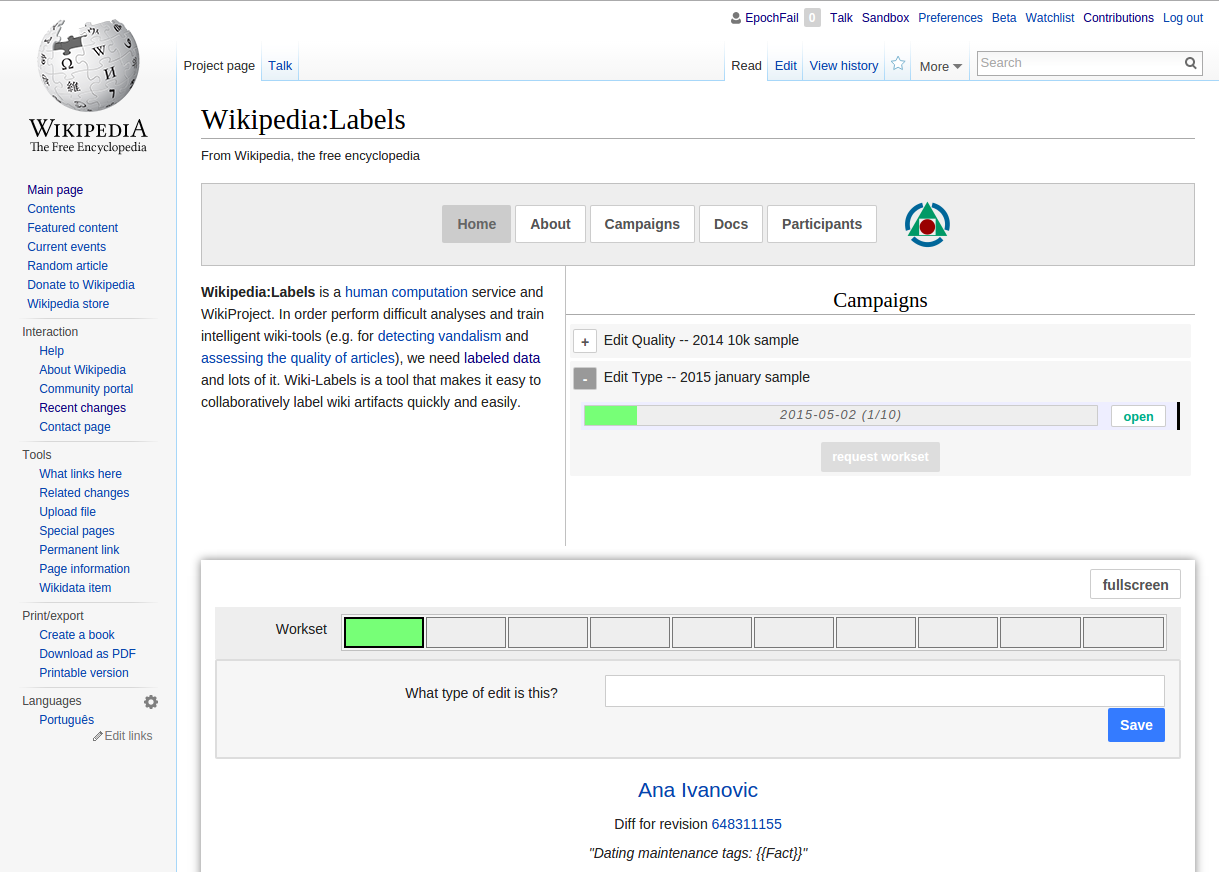
\includegraphics[width=.50\textwidth]{figures/Wiki_labels_gadget}
  \caption{The Wiki labels interface embedded in Wikipedia}
  \label{fig:wikilabels_screenshot}
\end{figure}

\leadin{Manual labeling campaigns with Wiki Labels}
We hold manual labeling by human Wikipedians as the gold standard for purposes of training a model to replicate human judgement.  By asking Wikipedians to demonstrate their judgement on examples from their own wikis, we can most closely tailor model predictions to match the judgements that make sense to these communities.  This contrasts with found data, which deceptively appears to be a better option because of its apparent completeness: every edit was either reverted or not.  In contrast, manual labeling has a high up-front expense of human labor.  To minimize that cost, we developed a high-speed, collaborative labeling interface called ``Wiki Labels\footnote{\url{http://enwp.org/:m:Wiki labels}}'' to allow Wikipedians to efficiently label large datasets.

For example, to supplement our models of edit quality, we replace the models based on ``reverted\_for\_damage'' found traces with judgments from a community labeling campaign, where we specifically ask labelers to distinguish ``damaging'' edits from ``good-faith'' edits. ``Good faith'' is a well-established term in Wikipedian culture\footnote{\url{https://enwp.org/WP:AGF}}, with specific local meanings that are different than their broader colloquial use---similar to how Wikipedians define ``consensus'' or ``neutrality''.  Using these labels we can build two separate models which allow users to filter for edits that are likely to be good-faith mistakes\cite{halfaker2017automated}, to just focus on vandalism, or to apply themselves broadly to all damaging edits.

\subsection{Dependency injection and interrogability}
One of the key features of ORES that allows scores to be generated in an efficient and flexible way is a dependency injection framework.  We use a dependency solver to determine what data is necessary for a scoring job and eventually compute the features used by a prediction model.

The flexibility provided by the dependency injection framework lets us implement a novel strategy for exploring \emph{how} ORES' models make predictions.  By exposing the features extracted to ORES users and allowing them to inject their own features, we can allow users to ask how predictions would change if the world were different.  Let's say you wanted to explore how ORES judges unregistered (anon) editors differently from registered editors.  Figure~\ref{fig:anon_injection} demonstrates two prediction requests to ORES.

\begin{figure*}[h]
\centering
\begin{subfigure}[t]{.5\textwidth}
  \makebox{\hrulefill}{
  \small
  \begin{verbatim}
  "damaging": {
    "score": {
      "prediction": false,
      "probability": {
        "false": 0.938910157824447,
        "true": 0.06108984217555305   }   }  }
  \end{verbatim}
  \hrule
  \normalsize}
  \caption{Prediction with \texttt{anon = false} injected}
  \label{fig:anon_injection_false}
\end{subfigure}~~
\begin{subfigure}[t]{.5\textwidth}
  \makebox{\hrulefill}{
  \small
  \begin{verbatim}
  "damaging": {
    "score": {
      "prediction": false,
      "probability": {
        "false": 0.9124151990561908,
        "true": 0.0875848009438092   }   }   }
  \end{verbatim}
  \hrule
  \normalsize}
  \caption{Prediction with \texttt{anon = true} injected}
  \label{fig:anon_injection_true}
\end{subfigure}
\caption{Two ``damaging'' predictions about the same edit are listed for ORES.  In one case, ORES is asked to make a prediction assuming the editor is unregistered (anon) and in the other, ORES is asked to assume the editor is registered.}
\label{fig:anon_injection}
\end{figure*}

Figure~\ref{fig:anon_injection_false} shows that ORES' ``damaging'' model concludes that the edit identified by the \emph{revision ID} of 34234210 is not damaging with 93.9\% confidence.  We can ask ORES to make a prediction about the exact same edit, but to assume that the editor was unregistered (anon). Figure~\ref{fig:anon_injection_true} shows the prediction if edit were saved by an anonymous editor.  ORES would still conclude that the edit was not damaging, but with less confidence (91.2\%).  By following a pattern like this for a single edit or a set of edits, we can get to know how ORES prediction models account for anonymity through experience with practical examples. Interrogability has also been used in creative new ways beyond bias explorations.  Some of our users have levered the feature injection system to expose \emph{hypothetical} predictions to support their work.  See the discussion of Ross's work recommendation tools in Section~\ref{sec:adoption_patterns}.
